\documentclass[11pt]{article}
\usepackage[review]{acl}
\usepackage{times}
\usepackage{latexsym}
\usepackage[T1]{fontenc}
\usepackage[utf8]{inputenc}
\usepackage{microtype}
\usepackage{inconsolata}
\usepackage{graphicx}
\usepackage{booktabs}
\usepackage{tabularx}
\usepackage{amsmath}
\usepackage{tikz}
\usetikzlibrary{arrows.meta,positioning}
\title{Beyond Mapping: A Theory-Grounded Framework for\protect\\Evaluating Analogical Transfer in Language Models}
\author{Anonymous ACL submission}
\begin{document}
\maketitle
\begin{abstract}
Language models can benefit from analogies without reliably transferring their relational structure. Additional explanation and answer cues can improve accuracy, while a net gain can conceal regressions. We introduce a theory-grounded diagnostic framework that operationalizes analogical reasoning through retrieval, mapping, schema induction, and adaptation. Explicit stage artifacts and information boundaries allow unsuccessful paths to be inspected and rerun after reference-informed upstream corrections. Three complementary evaluations link outcome measurement to process diagnosis. Scientific question-answering controls show that analogy gains need not exceed explanation or random-example effects. A factorial narrative experiment finds structure-dependent source-answer benefits, including transfer interactions of 14.24 and 12.94 percentage points for Llama-3.1-8B and 70B. In the diagnostic workflow, all initial GPQA failures occur at retrieval, yet 75.34\% of that failure cohort still reaches inadequate adaptation after upstream corrections. This separates the first visible barrier from the remaining difficulty. The framework enables more precise evaluation of helpful and harmful analogy use while distinguishing assisted continuation from independent model success.
\end{abstract}
\section{Introduction}
\label{sec:introduction}
Analogy supports reasoning by carrying a useful relational structure from a familiar source to a new target. In the classic fortress--radiation example, dividing an army across several routes suggests directing multiple low-intensity rays toward a tumor: individual paths remain safe, while their combined effect is sufficient at the target \citep{gick1980analogical}. The transferable content is a system of constraints and relations, including convergence and coordination. Sharing a topic or naming corresponding objects is insufficient.

Language models can generate examples, recognize analogies, and sometimes solve problems more accurately after receiving them. Analogical prompting uses self-generated problems and solutions \citep{yasunaga2024analogical}; teacher-generated analogies can also help scientific concept understanding \citep{yuan2024boosting}. However, random examples can produce comparable gains on some tasks \citep{qin2025relevant}. These findings raise a measurement question: \emph{relative to which controls, and through which operations, should an improvement count as evidence of analogical transfer?}

The question has two parts. First, the effect must be attributed carefully. Adding an analogy also adds text, explanation, and potentially answer-relevant knowledge. Comparing only against a prompt without examples cannot separate these factors. Even a positive average gain may combine repairs of incorrect answers with regressions on previously correct ones. Second, the process must be localized. A wrong answer can follow from inadequate sources, inconsistent correspondences, an unusable abstraction, or failure to apply a valid abstraction to target constraints. Final accuracy merges these failures. Conversely, a correct answer may be reached without using the analogy at all.

We address both parts through a theory-grounded framework for evaluating analogical reasoning in language models. Drawing on cognitive accounts of structural alignment, schema induction, and transfer, we operationalize four components: \textbf{retrieval}, \textbf{mapping}, \textbf{schema induction}, and \textbf{adaptation}. The model produces a separate output for each stage under an explicit information contract. We diagnose the first inadequate output in an unsuccessful trajectory, replace it with a reference-informed correction, and rerun the downstream stages with the same base model. This distinguishes an initial failure from additional failures that become visible after upstream repair.

The framework is supported by three connected studies. Phase~I examines the attribution of analogy effects in scientific question answering, including helpful and harmful answer transitions. Phase~II asks whether a solved, structurally corresponding source provides a selective advantage over a random source. Phase~III applies the stage framework to scientific and narrative problems to identify barriers to transfer. These phases answer different questions; together, they link controlled outcome measurement to process diagnosis.

Our contributions are:
\begin{itemize}
    \item A theory-grounded operational framework with explicit stage outputs and information boundaries, enabling diagnosis and cumulative intervention across retrieval, mapping, schema induction, and adaptation.
    \item A controlled analysis of analogy effects that distinguishes explanation, example length, relevance, textual mention, and item-level improvements and regressions.
    \item Empirical evidence for structure-dependent source-answer benefits, followed by a diagnosis showing that repairing early failures can reveal persistent downstream adaptation difficulties.
\end{itemize}
The stages are an externally imposed experimental decomposition. We neither claim to observe the model's hidden computation nor propose that every analogy must follow this temporal order. Our contribution is to make established theoretical distinctions testable in an auditable language-model workflow.

\section{A Theory-Grounded Diagnostic Framework}
\label{sec:framework}
\subsection{From cognitive distinctions to stage contracts}
Structure-mapping theory treats analogy as correspondence between relational systems rather than isolated attributes \citep{gentner1983structure}. Systematicity favors connected, especially causal, relations over disconnected local matches \citep{clement1991systematicity}; computational structure mapping makes consistency constraints explicit \citep{falkenhainer1989sme}. However, the availability of a source and the soundness of an inference from it are separable \citep{gentner1993roles,holyoak1987surface}. Comparing sources can yield a schema that abstracts the solution principle and its applicability conditions \citep{gick1983schema,gentner2003learning}. Applying that schema remains a further problem: target-specific constraints can defeat transfer even when an appropriate source is accessible \citep{novick1991math}.

We translate these distinctions into four externally controlled calls. Let $x$ denote the target, $r$ the solved sources, $m$ their mapping, $s$ a schema, and $a$ the adapted solution. The permitted information flow is
\begin{equation}
 \begin{aligned}
 r&=R(x), & m&=M(r),\\
 s&=S(m), & a&=A(x,s).
 \end{aligned}
 \label{eq:flow}
\end{equation}
Each call starts fresh; only the permitted recorded artifact passes forward. Figure~\ref{fig:framework} and Table~\ref{tab:contracts} describe the interfaces. The natural workflow never receives the target reference answer.

\begin{figure}[t]
\centering
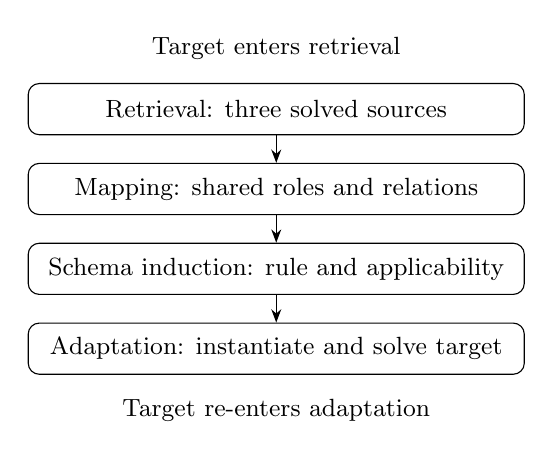
\begin{tikzpicture}[font=\small,>=Stealth,
 stage/.style={draw,rounded corners,align=center,minimum width=6.3cm,minimum height=.65cm},node distance=.35cm]
\node[stage] (r) {Retrieval: three solved sources};
\node[stage,below=of r] (m) {Mapping: shared roles and relations};
\node[stage,below=of m] (s) {Schema induction: rule and applicability};
\node[stage,below=of s] (a) {Adaptation: instantiate and solve target};
\draw[->] (r)--(m); \draw[->] (m)--(s); \draw[->] (s)--(a);
\node[above=.18cm of r] {Target enters retrieval};
\node[below=.18cm of a] {Target re-enters adaptation};
\end{tikzpicture}
\caption{An observable source-to-target workflow. Mapping compares sources; schema induction abstracts their mapped structure; adaptation reconnects the schema to the target. Each stage receives a restricted artifact rather than the entire preceding conversation.}
\label{fig:framework}
\end{figure}

\begin{table*}[t]
\centering
\small
\begin{tabularx}{\textwidth}{@{}p{2.3cm}p{3.65cm}X@{}}
\toprule
Stage & Permitted input & Required artifact and adequacy criterion \\
\midrule
Retrieval & Target and choices & Three solved sources with answers and explanations; sources must support a solution-relevant relational structure. \\
Mapping & Retrieval artifact only & Corresponding roles and relations across sources, source suitability, and material differences; correspondences must be consistent and informative. \\
Schema induction & Mapping artifact only & Abstract solution rule, roles, relations, applicability conditions, and limits; enough structure must remain to guide a new solution. \\
Adaptation & Target and necessary schema content & Instantiated roles, target-constraint checks, necessary adjustments, and a final answer supported by target evidence. \\
\bottomrule
\end{tabularx}
\caption{Stage contracts make theoretical distinctions operational. The raw target is withheld from the two middle stages, and raw sources are withheld from adaptation.}
\label{tab:contracts}
\end{table*}

\paragraph{Retrieval.}
This stage obtains three solved source problems. In our implementation, the model can generate them; ``retrieval'' names their functional role, not an observation of access to internal memory. Topical resemblance is insufficient: a source must preserve relations useful for solving the target, and its own explanation must be defensible.

\paragraph{Mapping.}
The model compares the retrieved sources with one another, recording shared roles, relations, useful examples, and consequential differences. It does not see the target. Consistency and connected relations matter more than a list of similar nouns. Alignable differences help distinguish incidental changes from discrepancies that invalidate transfer \citep{gentner1997mapping}.

\paragraph{Schema induction.}
The model sees only the recorded mapping. It must express an abstract solution rule together with conditions and limits. A schema should be general enough to cross domains while retaining the operations needed for a solution. The restriction tests whether the mapping artifact supports abstraction without rereading the original narratives.

\paragraph{Adaptation.}
The target re-enters with the schema, but without raw sources or the mapping. The model instantiates roles, adjusts domain-specific details, checks constraints, and answers. This is where the shared structure is connected to the actual target rather than merely described.

In the convergence example, the sources must retain that concentrated force is unsafe along a path, weak forces alone are insufficient, and coordinated forces combine at the goal. The mapping aligns this relational system; the schema states the conditions under which convergence works; adaptation checks whether the target satisfies them. ``Organize resources better'' is too general, while copying a source-specific object or answer position fails to instantiate the relation.

These boundaries define an experimental source-comparison-to-schema-to-target path. They may impose costs absent from ordinary prompting, and they are not a universal temporal model of cognition. Their value is to specify which artifact supports each next operation, making failures inspectable and replacements interpretable.

\subsection{Diagnosing first failure and downstream burden}
\label{sec:repair}
For each naturally unsuccessful trajectory, we inspect artifacts in stage order and record the first one inadequate for its assigned function. The label identifies the first observable failure in this workflow, not the unique hidden cause of the answer. An inadequate retrieval can mask whether the model would also fail to map, abstract, or adapt a good source.

We then replace only that artifact with a corrected one, retain earlier artifacts, and rerun downstream calls with the same base model. If the answer becomes correct, the continuation is rescued under the correction. Otherwise, the new path is inspected and the next inadequate artifact is corrected while prior corrections remain. This yields two distinct observations: the \emph{initial first-failure distribution}, and the \emph{burden revealed over cumulative repairs}. The latter can count one question at several stages.

GPT-6 Sol authors corrected artifacts with access to the target reference answer, an \emph{open-oracle} construction setting. Upstream corrections must be defensible under their stage contract and must not explicitly disclose the target answer. The base model continuing the workflow never receives the reference. This setting tests whether it can exploit solution-relevant upstream guidance; it does not measure autonomous source generation or an isolated causal effect of each stage.

Adaptation requires special treatment. A corrected adaptation artifact already includes the final answer and leaves no downstream model call. Agreement with the reference after that replacement is therefore not a rescue by the base model. We count genuine continuation only after retrieval, mapping, or schema corrections, and keep final oracle outputs separate. This distinction prevents an answer supplied by the correction procedure from being mistaken for successful transfer by the solver.

\section{Evaluation Design}
\label{sec:method}
The framework motivates three evaluation questions: do apparent analogy gains survive appropriate controls; do source solutions help selectively through intended correspondence; and which stage difficulties remain after upstream repair? The first two experiments examine outcomes under different source conditions. The third evaluates the imposed four-stage workflow. They provide complementary evidence, rather than a single benchmark score or one identical protocol.

\subsection{Tasks and response accounting}
GPQA Main contains 448 graduate-level science questions \citep{rein2023gpqa}, with 78 biology, 183 chemistry, and 187 physics items in the local version. We use Main rather than the 198-item Diamond subset. MuSR supplies murder mysteries, object placements, and team allocation \citep{sprague2024musr}. These tasks respectively require combining clues, tracking locations and agents' knowledge, and satisfying assignment constraints. GPQA often requires external scientific knowledge; MuSR provides much of the relevant evidence in its narratives, facilitating sources with changed entities but preserved solution relations.

Accuracy uses the reference choice. A recorded failed response or unextractable final answer is incorrect. Matched contrasts align identifiers, not file order. A missing question record is distinct from a recorded invalid response. Repeated calls to a question characterize execution variability, not additional independent questions. We interpret numerical patterns descriptively and distinguish run standard deviation from inferential uncertainty.

\subsection{Controls for apparent analogy benefits}
\label{sec:phase1method}
The scientific study compares concept-focused teacher analogies with explanations, random analogies, and solver-generated reasoning. DeepSeek V4 Flash creates the teacher content. Solvers are Llama-3.1-8B-Instruct, Qwen3-8B, Mistral-7B-Instruct-v0.3, and Gemma-4-31B-it. CoT and self-analogy provide strategies without an external teacher example \citep{wei2022cot,kojima2022zero}.

We compare a 300-word analogy with a 600-word analogy, and one, two, or three examples under a nominal 600-word total budget. Non-analogical explanations have 300- or 600-word budgets. Random examples come from the same or a different scientific domain. Each comparison has a specific purpose: length probes additional text; explanations probe whether benefits require analogical presentation; random sources probe the intended relation; and multiple examples probe the opportunity for comparative abstraction. The last comparison does not directly establish that a schema was induced.

A net gain can conceal both improvements and regressions. On the same items, with baseline $b$ and condition $c$, we measure
\begin{equation}
 p_c-p_b=H_{b\rightarrow c}-D_{b\rightarrow c},
 \label{eq:help-harm}
\end{equation}
where $H$ is the fraction changing from incorrect to correct and $D$ the fraction changing from correct to incorrect. Both use all shared items as denominator. We separately record explicit reference to the analogy, example, or teacher, including references that reject it. Mention and correctness are distinct observations; neither directly identifies valid structural use.

Llama, Qwen, and Mistral have 448 retained responses in each reported condition. Gemma has 435--447. Its overall accuracies can reflect changes in question composition; paired contrasts use shared identifiers. Appendix~\ref{app:execution} gives the counts and condition definitions.

\subsection{A factorial test of source-solution transfer}
\label{sec:phase2method}
For each selected MuSR target, GPT-5.6-Sol constructs a source with changed entities and context but intended shared solution relations. The generator sees the target reference answer; the solver does not. Sources contain a narrative, question, choices, and a separate correct source-answer field. Construction is checked for completeness, intended structural suitability, and absence of explicit target-answer disclosure, with manual review of difficult examples and a small model-based assessment rather than exhaustive human validation.

The experiment uses the 103 completed records available at execution: 61 murder mysteries, 21 object placements, and 21 team-allocation questions. This is neither full MuSR nor a documented representative random sample. Random controls reassign the same sources one-to-one among targets with equal choice counts, without self-assignment. Assignment reduces same-story and same-task matches where possible. Four five-choice object-placement items retain same-story controls because alternatives are unavailable. Random reassignment removes the designed correspondence, not every incidental useful relation.

We cross source type with source-answer availability: $A$ is corresponding/withheld; $B$ corresponding/provided; $C$ random/withheld; and $D$ random/provided. Withholding removes only the answer field, retaining source narrative, question, and choices. The target, neutral ``additional example'' label, instruction, temperature zero, and 2,048-token output ceiling are fixed. Selective source-answer benefit is
\begin{equation}
 \Delta_{\mathrm{transfer}}=(p_B-p_A)-(p_D-p_C).
 \label{eq:interaction}
\end{equation}
A positive interaction supports a greater answer benefit under intended correspondence. We report every cell because an interaction may combine improvement with damage to a control. Zero interaction can coexist with a useful corresponding source.

Llama-3.2-1B and 3B and Llama-3.1-8B and 70B Instruct have three runs per cell. Qwen3-14B and 32B have two. Provider and quantization differences prevent interpreting the comparison as a pure effect of model size. Random controls permute the same sources, making corpus-wide narrative lengths identical (mean 318.99 words), but not necessarily matching each pair or task. Source-choice shuffling updates answer indices. We compare $B$ on matching versus differing source/target answer positions to probe index following; the strata contain different questions, not controlled reorderings of the same target.

\subsection{Stage diagnosis and continuation tests}
\label{sec:phase3method}
We apply the workflow in Section~\ref{sec:framework} to Llama-3.1-8B-Instruct on 100 GPQA Main questions and 100 MuSR murder mysteries. Three solved sources are requested per target. We diagnose naturally unsuccessful workflows and perform the cumulative upstream repairs of Section~\ref{sec:repair}. The question is whether corrected intermediate guidance enables the base model to finish, and which inadequate stages emerge when it does not.

Human review covers 30\% of questions and associated outputs for logical coherence and correctness. The remaining cases have no human review; reference-informed correction is not equivalent to exhaustive validation. We report natural accuracy, the initial failure cohort, first-failure assignments, cumulative rescue, and overlapping stage burdens separately. All counts use the actual 100-item cohorts. Doubled display counts in some retained thesis graphics add no observations and are not used here.

\section{Results and Analysis}
\label{sec:results}
\subsection{The first failure can conceal the main remaining obstacle}
\label{sec:phase3results}
The diagnostic framework answers 27/100 GPQA questions and 57/100 murder mysteries correctly without corrections. The 73 GPQA failures are all first diagnosed at retrieval. The 43 murder-mystery failures begin at retrieval in 19 cases, mapping in 3, and adaptation in 21; none begins at schema induction. These are first-failure assignments within unsuccessful workflows, not unconditional stage error rates.

A first-failure label alone suggests that GPQA needs better sources and murder mysteries need better target application. Cumulative repair tests what this account leaves out. After retrieval correction, the same base model solves 17 of the 73 GPQA failures (23.29\%). Mapping correction does not add rescues, and schema correction adds one, bringing the total to 18/73 (24.66\%). For murder mysteries, the cumulative totals are 11, 14, and 15 of 43 failures after retrieval, mapping, and schema correction (25.58\%, 32.56\%, and 34.88\%). Figure~\ref{fig:repairs} follows the same initial failure cohorts.

\begin{figure}[t]
\centering
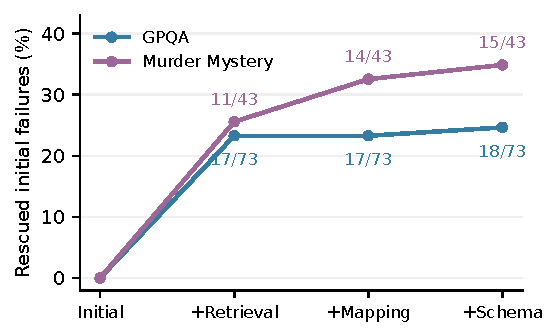
\includegraphics[width=\columnwidth]{figures/phase3_repairs.pdf}
\caption{Cumulative rescue of initially failed workflows after upstream corrections. Counts use the actual cohorts: 73 GPQA and 43 murder-mystery failures. Final gold adaptation is excluded because it supplies the answer rather than testing downstream base-model continuation.}
\label{fig:repairs}
\end{figure}

\paragraph{Failure migration and overlapping burden.}
After upstream corrections, adaptation remains inadequate for 55/73 GPQA failures (75.34\%) and 28/43 murder mysteries (65.12\%). GPQA also reveals mapping problems in 26/73 and schema problems in 15/73 over the correction history; murder mysteries reveal mapping problems in 6/43 and schema problems in 1/43. These burdens overlap because one trajectory can need several repairs. Appendix~\ref{app:states} separates mutually exclusive current states from overlapping cumulative burdens.

The distinction changes the interpretation of the initial diagnosis. Retrieval is the first barrier for every failed GPQA trajectory, but it is not the only barrier: most paths still fail after upstream guidance is corrected. In particular, moving a failure from retrieval to adaptation does not by itself indicate that the retrieval correction damaged the path. It can expose an operation that the original path never reached with an adequate input. Likewise, mapping correction can remove a visible deficiency without increasing final accuracy, because the schema or adaptation remains inadequate.

\paragraph{Rescue requires base-model continuation.}
Natural successes plus genuine continuation after upstream corrections give 45/100 correct GPQA answers and 72/100 correct murder mysteries. These are assisted workflow outcomes. Replacing adaptation with a reference-informed final answer is excluded: that intervention supplies the result instead of testing the solver's ability to finish. Reporting it as model rescue would erase precisely the downstream difficulty that the framework identifies.

The domain contrast is compatible with the task demands. Scientific questions require external knowledge to understand the target and obtain useful sources. Murder mysteries provide many relevant facts but require instantiating relations under particular story constraints. These results do not identify hidden mechanisms; they show why observable source adequacy and target adaptation need separate assessment.

\subsection{Solved sources can support structure-dependent transfer}
\label{sec:phase2results}
To establish that sources can help through more than their mere presence, we examine the factorial source-answer test in Table~\ref{tab:phase2}. Llama-1B gains 5.50 points when either the corresponding or random source answer is provided, yielding zero mean interaction. Llama-3B gains about 13.92 points from corresponding source content in both answer settings, but the answer adds the same 2.91 points in either source type. Its zero interaction therefore does not mean the corresponding source is useless; it means the observed answer benefit is not selective.

\begin{table*}[t]
\centering
\small
\begin{tabular}{@{}lrrrrr@{}}
\toprule
Model & $A$: true/no answer & $B$: true/answer & $C$: random/no answer & $D$: random/answer & $\Delta_{\mathrm{transfer}}$ \\
\midrule
Llama-3.2-1B & $38.51\pm1.48$ & $44.01\pm0.56$ & $38.51\pm2.02$ & $44.01\pm0.56$ & $0.00$ \\
Llama-3.2-3B & $54.05\pm1.48$ & $56.96\pm0.56$ & $40.13\pm1.12$ & $43.04\pm1.48$ & $0.00$ \\
Llama-3.1-8B & $52.10\pm3.68$ & $65.70\pm3.41$ & $52.43\pm1.94$ & $51.78\pm7.35$ & $+14.24$ \\
Llama-3.1-70B & $59.22\pm3.88$ & $72.17\pm8.76$ & $53.07\pm2.24$ & $53.07\pm2.02$ & $+12.94$ \\
\midrule
Qwen3-14B & $66.02\pm4.12$ & $75.24\pm0.69$ & $60.68\pm2.06$ & $60.68\pm3.43$ & $+9.22$ \\
Qwen3-32B & $68.93\pm2.75$ & $74.27\pm0.69$ & $65.53\pm2.06$ & $58.25\pm2.75$ & $+12.62$ \\
\bottomrule
\end{tabular}
\caption{Factorial transfer accuracy (\%, mean $\pm$ run SD) on the same 103 MuSR targets in every cell. Llama has three runs; Qwen has two. Interactions are in percentage points, computed from unrounded run-level values; rounding displayed cells can produce small discrepancies. SD is not an inferential confidence interval.}
\label{tab:phase2}
\end{table*}

Llama-8B and 70B show a different pattern. The 8B model gains 13.59 points from the corresponding answer and changes by $-0.65$ points with the random answer, giving a 14.24-point interaction. The 70B model gains 12.94 points from the corresponding answer and none from the random answer. These results support structure-dependent use of source answers under the tested protocol. They do not show that every correct answer used the source or that transfer grows monotonically with model size.

The pattern also appears outside the Llama family. Qwen-14B gains 9.22 points from the corresponding answer, with no change in the random-answer mean. Qwen-32B combines a 5.34-point corresponding-answer gain with a 7.28-point random-answer loss, giving a 12.62-point interaction. Its larger interaction does not mean a larger benefit from the valid guide: part of the difference comes from damage in the control. The individual cells are essential to the interpretation.

\paragraph{Transferring an answer role is different from copying an index.}
Llama-1B achieves 88.24\% accuracy when source and target correct-answer positions match and only 0.64\% when they differ. Together with equal answer gains for corresponding and random sources, this suggests predominant index following. Llama-8B and 70B retain 57.05\% and 65.38\% accuracy in the different-position stratum, compared with 74.51\% and 79.08\% in the matching stratum. Their performance is compatible with more than index copying, although position sensitivity persists. Since the strata contain different questions, this check supports rather than independently establishes the factorial interpretation.

Thus, there is positive evidence for selective source use in several evaluated models, alongside substantially different behaviors in smaller models. The framework is useful in this setting because a capacity demonstrated under a supplied source does not guarantee that a model can obtain, abstract, and apply an adequate source on its own.

\subsection{Aggregate gains and textual mention are insufficient measures}
\label{sec:phase1results}
The scientific controls explain why the stronger attribution test and stage diagnosis are needed. In Table~\ref{tab:phase1}, the concept-focused 300-word analogy does not outperform both random controls for any solver. Llama performs slightly better with a same-domain random source, Qwen matches it, and Mistral trails both random controls. Gemma lies between its controls, with the additional caveat of differing retained sets. The intended example relation does not yield a general advantage in final accuracy.

\begin{table*}[t]
\centering
\small
\begin{tabular}{@{}lrrrr@{}}
\toprule
Condition & Llama-8B & Qwen-8B & Mistral-7B & Gemma-31B \\
\midrule
Analogy, 300 words & 30.80 & 36.61 & 27.01 & 65.39 \\
Analogy, 600 words & 31.25 & 36.83 & 28.79 & 68.69 \\
Two analogies, $2\times300$ words & 31.92 & 35.27 & 30.58 & 69.00 \\
Three analogies, $3\times200$ words & 31.03 & 39.73 & 26.56 & 69.61 \\
Non-analogical explanation, 300 words & 31.03 & 37.72 & 27.68 & 68.25 \\
Non-analogical explanation, 600 words & 30.58 & 36.61 & 25.89 & 68.47 \\
Random same-domain analogy, 300 words & 31.25 & 36.61 & 27.68 & 64.85 \\
Random different-domain analogy, 300 words & 29.69 & 39.73 & 28.13 & 67.12 \\
Chain-of-thought & 32.14 & 42.19 & 16.96 & 66.52 \\
Self-analogy & 28.79 & 43.30 & 22.54 & 64.06 \\
\bottomrule
\end{tabular}
\caption{Scientific question-answering accuracy (\%) on GPQA Main. Llama, Qwen, and Mistral have 448 retained responses per condition. Gemma has 435--447, so its overall contrasts can also reflect changes in the retained question set. Recorded responses without a final answer are incorrect.}
\label{tab:phase1}
\end{table*}

\paragraph{The comparison determines the claim.}
Mistral's teacher analogy raises accuracy from 16.96\% under CoT to 27.01\%. Yet a 300-word non-analogical explanation reaches 27.68\%. A gain against CoT therefore does not establish a benefit requiring analogical presentation. Llama's teacher analogy and explanation both trail its CoT baseline. Qwen's self-analogy reaches 43.30\%, compared with 42.19\% for CoT and 36.61\% for the teacher analogy. These are effects of particular assistance and prompting conditions, not interchangeable measures of transfer.

Longer or more numerous examples also fail to provide a uniform benefit. Doubling analogy length adds 0.45 points for Llama and 0.22 for Qwen. At a nominal total of 600 words, Mistral's one-, two-, and three-example accuracies are 28.79\%, 30.58\%, and 26.56\%, while explicit mentions increase from 12.05\% to 19.42\% and 29.24\%. Increased engagement with examples in the output is not direct evidence that a usable schema was induced.

\paragraph{Net improvement can coexist with damage.}
On the same 448 items, Mistral's 300-word analogy repairs 86 CoT errors (19.20\% of all items) while making 41 previously correct answers incorrect (9.15\%). The 45-item net gain is 10.04 percentage points. Two 300-word examples repair 105 answers and damage 44. Figure~\ref{fig:transitions} makes both directions visible. These are condition-associated changes: differing instructions and similar changes under random controls prevent assigning every regression to a faulty analogical mapping.

\begin{figure}[t]
\centering
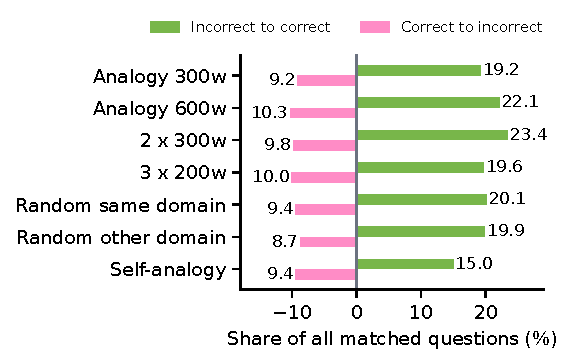
\includegraphics[width=\columnwidth]{figures/phase1_transitions.pdf}
\caption{Mistral transitions relative to CoT on the same 448 questions. Improvements and regressions use all shared items as denominator. Their difference is the net accuracy change.}
\label{fig:transitions}
\end{figure}

\paragraph{Mention is neither successful transfer nor its necessary trace.}
Qwen mentions the 300-word example in 31.70\% of all responses, compared with 8.31\% for Gemma despite Gemma's higher accuracy. Qwen's mention rates within correct and incorrect answers are 31.10\% and 32.04\%. Explicit reference can accompany either outcome, and absence of reference does not prove that the example had no effect. Diagnosing the actual intermediate artifacts gives a more specific question: did the source provide an adequate relation, was it preserved in the schema, and was it applied under the target constraints?

Together, these evaluations establish a hierarchy of evidence rather than a single ranking. Outcome changes show practical effects; controls narrow their attribution; selective source-answer gains support transfer under an intended correspondence; and stage interventions reveal what prevents that process from completing. The claim supported by each measurement depends on the information and operations it actually tests.

\section{Related Work}
\label{sec:background}
\paragraph{Identifying analogies.}
ARN and AnaloBench evaluate analogy identification in narratives under variations in surface similarity and context \citep{sourati2024arn,ye2024analobench}. Recognizing a corresponding source is informative, but does not establish that its solution can be adapted to a target. Our framework preserves this distinction by separating source adequacy from later abstraction and application. The theoretical connection follows the broader effort to relate cognitive accounts of analogy to relational understanding in NLP \citep{petersen2026modelling}; our contribution is an executable diagnostic protocol with restricted interfaces and cumulative repairs.

\paragraph{Using analogies for problem solving.}
Analogical prompting generates relevant exemplars before solving the target \citep{yasunaga2024analogical}. SCUA evaluates teacher-generated analogies as explanations of scientific concepts \citep{yuan2024boosting}. These approaches establish utility under their respective settings, but example quality, additional explanation, and target-solving instructions can change together. We compare concept explanations against specific controls and then construct a factorial source-answer test to distinguish source content benefits from selective solution transfer.

\paragraph{Attributing analogy effects.}
\citet{qin2025relevant} show that random self-generated examples can also help, challenging an interpretation based on relevance alone. Our scientific results reinforce this measurement concern while exposing helpful and harmful transitions hidden by a mean. The narrative experiment provides complementary positive evidence by testing answer availability under intended correspondence and random reassignment of the same source corpus. Finally, stage diagnosis moves from whether a source condition helps to which observable operation remains inadequate. We do not claim to originate multi-component accounts of analogy or to infer hidden cognitive processes from generated text.

\section{Conclusion}
An analogy's evaluation should distinguish outcome changes, selective source benefit, and deficiencies in an explicit transfer attempt. We introduce a theory-grounded framework that makes source construction, mapping, schema induction, and adaptation inspectable through restricted artifacts. Controlled outcomes and a factorial source-answer study motivate this distinction; recorded continuations show that first-stage assignments do not describe the full corrected path. The framework supports a more precise diagnostic account while keeping natural performance, oracle-assisted continuation, and claims about hidden reasoning separate.

\clearpage
\section*{Limitations}
Our findings concern English multiple-choice scientific and narrative tasks. The narrative transfer cohort is the 103 completed items available during execution, not a documented representative sample. Scientific assistance conditions differ in content, instructions, and nominal word budgets; they are not a pure manipulation of analogy. Gemma's retained question counts differ by condition. Llama's final scientific set combines an initial provider run with recovery of failed requests through another provider. Family, size, quantization, and endpoint differences cannot be cleanly separated.

The target-story resampling intervals are conditional descriptions under a fixed corpus, source assignment, and prompt. They do not capture regeneration of sources, variation across random permutations, annotation uncertainty, or all cross-question dependencies introduced by reusing source material across cells. We do not use them for multiplicity-adjusted hypothesis tests or universal scaling claims. The valid-output subset is selected after generation. Answer-position strata compare different items and do not control their difficulty. Oracle-aware source generation and incomplete structural validation limit the interpretation of selective benefits.

The primary stage trajectories cover one base model on two 100-item cohorts and are retained aggregate reports. Natural direct/staged outcomes for a second model and one recoverable schema case broaden context, but do not establish a fully validated second-model replication of stage frequencies. Human review covers 30\% of primary-study questions and outputs, with no inter-annotator agreement estimate. Thus inspection labels should be read as case-study assignments, not ground-truth causal mechanisms. The observable artifacts may be post-hoc products of target reasoning; neither structured output nor self-reported use establishes faithfulness.

Reference authors know the target key. References may indirectly encode answer guidance even without explicit disclosure, and correction changes content, style, and potentially length. Cumulative replacement and fresh downstream sampling do not identify independent stage effects. Unchanged-artifact repeats, matched rephrasing controls, blind reference audits, and interface ablations are not reported. Final adaptation replacement supplies an answer, so it is excluded from base-model continuation success. Direct answering and the staged workflow are not compute-matched; no efficiency or state-of-the-art claim is made.

\section*{Ethical Considerations}
We use existing scientific and synthetic narrative benchmarks and generated sources. A persuasive analogy can omit a decisive constraint and damage an otherwise correct answer, so benchmark improvements alone do not justify scientific or educational deployment. Dataset and model use remain subject to their licenses and service terms. Generative AI assisted the English manuscript, LaTeX, and offline analysis implementation; authors remain responsible for verifying text, sources, numerical provenance, and analysis. Experimental model use for source generation and oracle-authored references is described in the method. No new model calls or human annotations were added during this manuscript revision.

\bibliography{custom}
\appendix
\section{Execution and Evaluation Details}
\label{app:execution}
This appendix specifies condition construction and accounting. The accompanying analysis inputs contain de-identified outcome metadata and retained aggregates. They do not constitute a new annotation of intermediate correctness. Archived experiments and the offline analyses in this manuscript are distinct: no model calls were added for this revision.

\subsection{Scientific conditions and complete accuracies}
Condition~1 is the main-concept 300-word teacher analogy; 2 is one 600-word analogy; 3 and 4 are two 300-word and three 200-word examples. Conditions~5 and 6 are 300/600-word explanations. Conditions~7 and 8 are random same-domain/other-domain analogies. Condition~20 requests CoT; 21 requests solver-generated analogy with a 600-word generation ceiling. The broader archive includes an unrestricted-concept condition~0, which is not the selected analogy here.

\begin{table*}[t]
\centering\small
\begin{tabular}{@{}lrrrr@{}}
\toprule
Condition & Llama-8B & Qwen-8B & Mistral-7B & Gemma-31B \\
\midrule
Analogy, 300 words & 30.80 & 36.61 & 27.01 & 65.39 \\
Analogy, 600 words & 31.25 & 36.83 & 28.79 & 68.69 \\
Two analogies, $2\times300$ words & 31.92 & 35.27 & 30.58 & 69.00 \\
Three analogies, $3\times200$ words & 31.03 & 39.73 & 26.56 & 69.61 \\
Non-analogical explanation, 300 words & 31.03 & 37.72 & 27.68 & 68.25 \\
Non-analogical explanation, 600 words & 30.58 & 36.61 & 25.89 & 68.47 \\
Random same-domain analogy, 300 words & 31.25 & 36.61 & 27.68 & 64.85 \\
Random other-domain analogy, 300 words & 29.69 & 39.73 & 28.13 & 67.12 \\
Chain-of-thought & 32.14 & 42.19 & 16.96 & 66.52 \\
Self-analogy & 28.79 & 43.30 & 22.54 & 64.06 \\
\bottomrule
\end{tabular}
\caption{Full scientific accuracies (\%). Llama, Qwen, and Mistral retain all 448 question responses per condition. Gemma has differing retained question sets, so small column differences can include composition effects.}
\label{tab:phase1}
\end{table*}

Gemma response counts for conditions 1, 2, 3, 4, 5, 6, 7, 8, 20, and 21 are respectively 445, 444, 442, 441, 441, 444, 441, 444, 435, and 447. Correctness transitions use shared identifiers; a missing record differs from a retained response with no valid answer. Llama's final scientific set combines DeepInfra output with AvalAI recovery of failed requests. All 448 items remain in its accuracy denominator.

At a nominal 600-word total, Mistral's one-, two-, and three-example accuracies are 28.79\%, 30.58\%, and 26.56\%; explicit mentions are 12.05\%, 19.42\%, and 29.24\%. Thus additional references in output do not independently validate schema induction. The mention screen is lexical and includes rejecting an example.

\subsection{Narrative source construction}
Sources contain narrative, question, choices, and answer fields. Generation preserves choice count, requests one correct source option, and caps source narrative length below 1,000 words. Source-choice reordering uses seed 20260901 and random assignment uses seed 20260903; the source key is updated after reordering. Withholding deletes only the answer field. An earlier condition that also removed source choices is excluded from the factorial comparison.

Corresponding/random narrative lengths average 371.41/371.41 words for murder, 189.14/228.76 for objects, and 296.57/256.95 for teams. Both full-corpus means are 318.99 words because random assignment uses the same source set. Equality at corpus level does not imply item- or task-level length matching. The four same-story controls are recorded in the assignment metadata and excluded together from all cells in the sensitivity analysis.

Small Llama models use Cloudflare, Llama-8B uses Novita FP8, and Llama-70B uses DeepInfra; Qwen uses DeepInfra FP8. These deployments do not isolate model size from infrastructure. Output extraction status is retained separately from correctness.

\subsection{Conditional uncertainty and sensitivity}
\label{app:sensitivity}
For item $i$, average correctness over saved runs to obtain $\bar y_{ic}$ for cell $c$. Its contrast is $d_i=\bar y_{iB}-\bar y_{iA}-\bar y_{iD}+\bar y_{iC}$. The reported interaction is $100\sum_i d_i/n$. Group identifiers combine task and story ID. Each bootstrap draw samples 88 groups with replacement, retaining every question in a selected group and all its cells/runs. The draw's statistic divides by its number of sampled questions, which may vary with cluster size. The percentile interval uses 20,000 draws and seed 20261012.

This procedure holds constructed sources and the permutation fixed. Source material appears in different cells across questions; resampling target groups does not address every dependency or all possible new assignments. The intervals describe conditional resampling stability, not a confirmatory causal test. No adjustment for exploring six model interactions is applied.

\begin{table*}[t]
\centering\small
\begin{tabular}{@{}lrrrrrrr@{}}
\toprule
Model & Invalid $A$ & Invalid $B$ & Invalid $C$ & Invalid $D$ & Valid-all $n$ & Valid-all $\Delta$ & Exclude same-story $\Delta$ \\
\midrule
Llama-1B & 24 & 14 & 29 & 4 & 80 & 7.92 & $-0.34$ \\
Llama-3B & 2 & 4 & 0 & 5 & 98 & $-0.34$ & $-1.35$ \\
Llama-8B & 0 & 1 & 0 & 0 & 102 & 14.05 & 13.80 \\
Llama-70B & 13 & 9 & 8 & 7 & 88 & 14.02 & 13.13 \\
Qwen-14B & 24 & 23 & 40 & 39 & 58 & 12.07 & 9.60 \\
Qwen-32B & 13 & 19 & 20 & 25 & 65 & 10.00 & 12.63 \\
\bottomrule
\end{tabular}
\caption{Sensitivity diagnostics. Invalid counts are response events, out of 309 per Llama cell or 206 per Qwen cell. Valid-all keeps questions valid in every cell and execution, a post-output selected subset. Excluding same-story controls uses the same 99 questions in all cells. Interactions are percentage points.}
\label{tab:sensitivity}
\end{table*}

In $B$, 51 questions have matching source/target answer indices and 52 differ. Three Llama runs yield 153/156 events, not that many independent questions. Correct matching/differing counts are 135/1 for 1B, 93/83 for 3B, 114/89 for 8B, and 121/102 for 70B. The differing strata may differ in difficulty; these counts are not a randomized reordering experiment.

\section{Diagnostic Accounting and Recoverable Interfaces}
\label{app:states}
\begin{table}[t]
\centering\small
\begin{tabular}{@{}lrrrrr@{}}
\toprule
State & Success & R & M & S & A \\
\midrule
\multicolumn{6}{l}{GPQA: 73 initial Llama errors} \\
Initial & 0 & 73 & 0 & 0 & 0 \\
After R & 17 & 0 & 26 & 7 & 23 \\
After M & 17 & 0 & 0 & 15 & 41 \\
After S & 18 & 0 & 0 & 0 & 55 \\
\midrule
\multicolumn{6}{l}{Murder: 43 initial Llama errors} \\
Initial & 0 & 19 & 3 & 0 & 21 \\
After R & 11 & 0 & 6 & 0 & 26 \\
After M & 14 & 0 & 0 & 1 & 28 \\
After S & 15 & 0 & 0 & 0 & 28 \\
\bottomrule
\end{tabular}
\caption{Retained aggregate state accounting. Each row conserves its original error cohort. ``After'' denotes cumulative replacement; successful earlier continuations are carried forward. Final oracle adaptation is excluded.}
\label{tab:states}
\end{table}

The overlapping stage burdens are R/M/S/A = 73/26/15/55 for GPQA and 19/6/1/28 for murder. Summing these would count paths more than once. These values come from retained aggregate diagnostics. Some restored graphics multiply observed counts by two; the present analysis returns to 100 questions per task and never treats scaled counts as additional observations. Older 50-item reports are not mixed with the 100-item results.

The Llama identifier is \texttt{cf.llama-3.1-8b-instruct-fast}; the contextual second model is \texttt{deepseek-v4-flash}. Natural direct/staged transitions (incorrect-to-correct / correct-to-incorrect) are 15/13 and 10/16 for Llama GPQA/murder, and 19/14 and 11/12 for DeepSeek. These are question-matched observed outputs, not a token-matched architecture comparison.

A recoverable individual DeepSeek case is \texttt{musr\_murder\_mystery:87:0}. The saved continuation is marked completed and oracle-assisted, dated 2026-10-02. Its chain records original base-model R and M, a strong manual S replacement, and base-model A rerun. The schema reference contrasts method-specific evidence with generic motive/access. The extract preserves the empty original schema, the initial unresolved schema check, the replacement, provenance, and answer A-to-B transition. The stored ``strong manual replacement'' label is a provenance label, not proof of independent human validation or verified authorship by a particular reference model.

\subsection{Recorded input-key audit}
For the 400 natural staged cases in the matched Llama/DeepSeek cohorts, recorded prompt objects expose only the expected input keys: R receives \texttt{target, source\_count}; M receives \texttt{sources}; S receives \texttt{mapping\_package}; and A receives \texttt{target, schema}. The audit covers every recorded attempt. It finds four stage templates, all tagged \texttt{1.1-dev-6}. Among 400 workflows, 391 record four attempts, five record five, two record six, one records seven, and one records eight. These counts include retries and exclude oracle continuations.

This mechanical audit validates recorded explicit interfaces, not the correctness of outputs, absence of indirect target information in generated sources, or provider-side state. The recorded M task includes suspect/motive examples even for GPQA. We preserve this historical wording and report the possible domain bias rather than silently changing a prompt and attributing old outcomes to the new wording.

\subsection{Offline analysis package}
The bundled outcome metadata, source-assignment IDs, stage templates, aggregate states, and compact case extract support reproducing the new offline statistics and both figures without model calls. \texttt{scripts/analyze\_retained\_results.py} checks cohort sizes, matching identifiers, four-cell coverage, and the permutation; \texttt{scripts/build\_figures.py} uses bundled counts. A rendering adapter accepts a caller-supplied stateless completion function and instantiates the recorded four contracts without a built-in API connection; it is not the historical retry implementation. The analysis manifest records input hashes. This package reproduces reported summaries, not the original live API experiments or a fresh semantic annotation of all intermediate artifacts. Historical model aliases and human review details limit complete live replication.

\end{document}
